\documentclass[paper-main.tex]{subfiles}


\begin{document}
% I've rephrased the first part of this section a lot and provide some justification below
% I think we need to lead with the details of the signal here (similar to the last section), not the specifics of the data analysis as the issues seem confused here. The fact that long data sets are analysed is not because of the signal wandering, if anything that's an argument against analysing long data sets to make detection easier, it's because the signal has low amplitude. Also what is the justification of the "(but not always)" statement, do you have a reference? - hannah
% Hmm, not sure where I got "(but not always)" from but if I didn't note it down then then I have no idea why now. Re: long time sensing, I was trying to justify that frequencies can wander but I prefer your rewrite. - James


\begin{comment}
Continuous wave searches, such as in Refs.~\cite{SuvorovaEtAl:2016,SuvorovaEtAl:2017,SearchTwoSpecS6:2017,SunEtAlSNR:2018,JonesSun:2020}, are often (but not always) performed on long datasets (months to years in duration). 
The frequency of a continuous wave signals may wander significantly over this timescale, due to stochastic internal processes in the superfluid interior of isolated neutron stars~\cite{MelatosDouglassSimula:2015,Jones:2010} or variable accretion flows onto a neutron star from a stellar companion (e.g. as in LMXBs)~\cite{BildstenTB:1998}. In this context, wandering ``significantly'' means ``across multiple frequency bins'', where the typical width of a frequency bin is the reciprocal of the total observing time~\cite{JKS:1998,ScoX1O2Viterbi:2019}.
The audio analogue to these continuous wave signals is a tone that wanders in frequency; a note that changes pitch. Here, we adapt the data analysis technique used to search for slowly wandering continuous waves signals from spinning neutron stars in aLIGO and aVirgo data~\cite{SuvorovaEtAl:2016,SuvorovaEtAl:2017}. 
\end{comment}



Unlike the signal considered in Section~\ref{sec:single_tone}, continuous gravitational waves may not be monochromatic.
A continuous-wave signal may wander slowly (and randomly) in frequency over time, due to stochastic internal processes in the superfluid interior of isolated neutron stars\cite{MelatosDouglassSimula:2015,Jones:2010}, or variable accretion flows from a stellar companion for neutron stars in binaries as in LMXBs~\cite{BildstenTB:1998}. 
The audio analog is a tone that wanders in frequency: a note that changes in pitch. 



We first demonstrate why a Fourier transform applied to the whole dataset (as in Section~\ref{sec:single_tone}) is not well suited to the wandering frequency case.
As shown in Fig.~\ref{fig:viterbi_comparison_webcam_spectrum}, the signal is spread across multiple frequency bins, making it challenging or in some cases impossible to detect.
%A different means of detection is needed for a signal which has a randomly wandering frequency. 

In continuous wave searches, the wandering frequency problem is solved using the Viterbi algorithm~\cite{Viterbi:1967}, which can track the signal's frequency over time.
The analysis described and presented in this section is directly inspired by real continuous-wave search methods~\cite{SuvorovaEtAl:2016,SuvorovaEtAl:2017}. 
In section~\ref{sec:realCWSearches} we briefly review the analysis method used by LIGO and Virgo, in Section~\ref{sec:viterbi} we describe the methods as applied in this work, and in section~\ref{sec:wanderingResults} we show results for recovering a wandering frequency signal using the table-top interferometer. 

\begin{figure}
	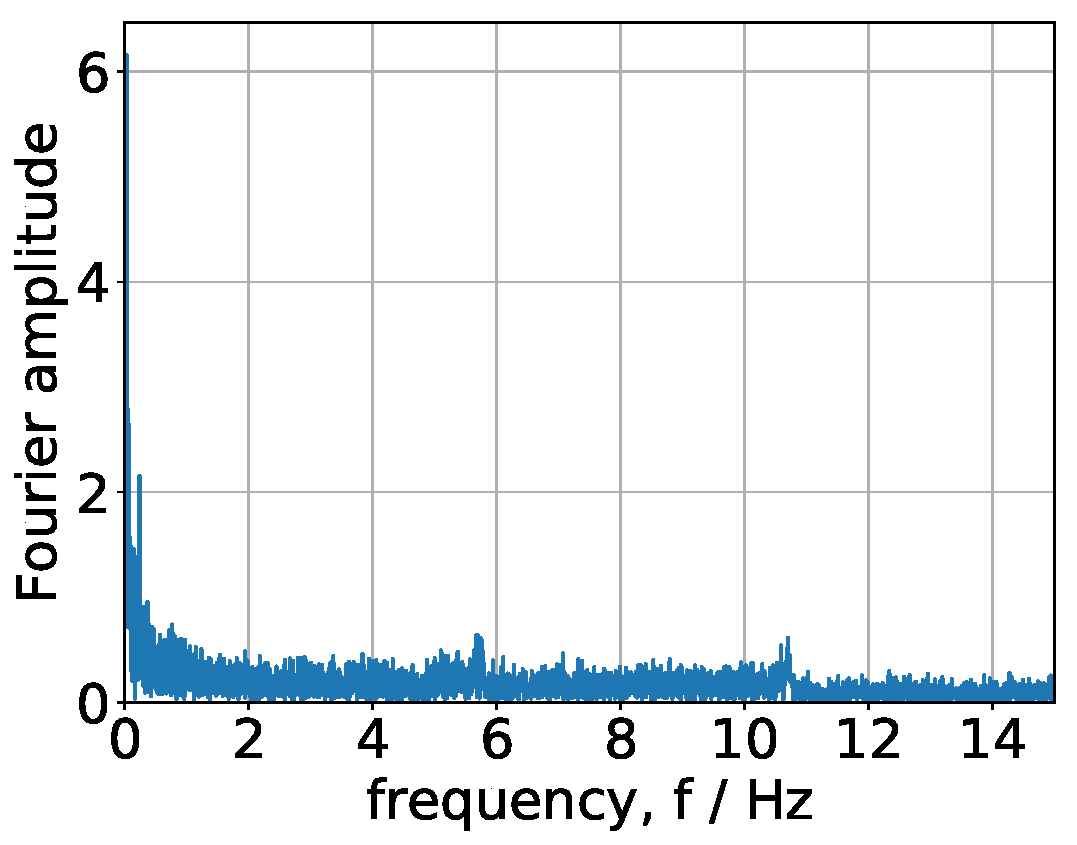
\includegraphics[width=.45\textwidth]{figures/viterbi_comparison_entire_spectrum_viterbi_test_webcam.pdf}
	\caption{\label{fig:viterbi_comparison_webcam_spectrum}
Fourier amplitude identical to that shown in Fig.~\ref{fig:webcam_spectrum}, except using a signal which has a slowly changing frequency instead of a constant frequency signal.
The signal is spread between many frequency bins. 
We see peaks at $5.7\,{\rm Hz}$ and $10.7\,{\rm Hz}$ and refer the reader forward to Fig.~\ref{fig:viterbi_overlay} to see the frequency evolution of this signal. 
A single Fourier transform of the entire dataset is not well suited to detecting signals with wandering frequencies.
% just making this a little more concise 
%Why we use the Viterbi algorithm to recover wandering frequency signals: Here we plot the Fourier amplitude of the intensity pattern against frequency as in Fig.~\ref{fig:webcam_spectrum} for the entire timeseries of the wandering frequency signal in Fig.~\ref{fig:viterbi_overlay}. Instead of resolving definite peaks like the constant frequency signal shown in Fig.~\ref{fig:webcam_spectrum}, we only see inconclusive peaks at 5.7~Hz and 10.7~Hz that correspond to the long amount of time that the wandering frequency spends near those values and/or its amplitude there, as seen in the pink dots in Fig.~\ref{fig:viterbi_overlay}. With the signal spread out over the frequency bins, we are unable to reliably detect it above the noise and therefore we use the Viterbi algorithm instead.
%The large values at low frequencies below 0.1~Hz are similar to those in Fig.~\ref{fig:webcam_spectrum} and can be ignored as they are likely inaccurate due to the short length of the signal relative to their period (i.e.\ 300~s only contains 30~periods of a 0.1~Hz signal), but this feature would require further research to fully determine its origin. %maybe could be from the long period (100~s) variation?
}
\end{figure}


\subsection{Continuous wave analysis with real data}
\label{sec:realCWSearches}

The methods used here are  inspired by LIGO-Virgo continuous wave searches. 
For further details on these methods see Refs.~\cite{SuvorovaEtAl:2016,SuvorovaEtAl:2017} and for searches performed using them see Refs.\cite{ScoX1O2Viterbi:2019, ScoX1ViterbiO1:2017, MillhouseStrangMelatos:2020, JonesSun:2020, MiddletonEtAlO2LMXBs:2020, PostMergerRemnantSearch:2019, SunEtAlSNR:2018, viterbi_application}. \han{check for new papers - add Deeksha's paper}
For other continuous wave search analyses not discussed here, see for example Refs.\han{todo}\cite{} and for further information on searching for transient gravitational wave signals, see for example Refs.~\cite{MillhouseEtAl:2018, Mohanty:2017, AddessoEtAl:2016, ThraneCoughlin:2014, ThraneEtAl:2011, CandesEtAl:2008, ChassandeMottinArchana:2006, AndersonBalasubramanian:1999}.


Continuous-wave searches are performed on long datasets, months to years in duration. 
The frequency of the signal can wander significantly over the observation period. 
In this context, ``significantly'' means across multiple frequency bins, where the typical width of a frequency bin is the reciprocal of the total observation time~\cite{JKS:1998,ScoX1O2Viterbi:2019}.
%One method to search for a wandering signal is to split the timeseries data into several shorter segments which are analyzed individually.


In Refs.~\cite{SuvorovaEtAl:2016,SuvorovaEtAl:2017}, a hidden Markov model is used to search for continuous gravitational waves. 
In a Markov process, the current state depends only on the previous state (in this case the state is the frequency of the signal). 
In a hidden Markov model, the frequency state of the signal is unknown, or hidden, and can undergo transitions at discrete times. 
The transitions are Markovian in that the hidden state (i.e.\ frequency) of the system at any time depends solely on its state at the previous time. 


A detection statistic relates the observed data to the hidden state and quantifies the likelihood of a signal being present in the data at each frequency and time bin.
This likelihood is also called the emission matrix in gravitational-wave literature.  
In gravitational-wave data analysis, the detection statistic gives the likelihood of a signal given the antenna beam pattern of the detector, which varies as the Earth rotates and orbits the Sun~\cite{JKS:1998}.
If searching for continuous waves from a neutron star in a binary (such as an LMXB), the Doppler modulation of the source also needs to be taken into account and a different detection statistic is used~\cite{SuvorovaEtAl:2017}. 


In continuous wave searches, a physical model of the target informs how far the frequency of the signal can wander over at each time. 
This is called the transition probability matrix. 
In LMXB searches, the transition matrix allows the signal frequency to (a) stay in the same frequency bin, (b) move up a single frequency bin, or (c) move down a frequency bin at each time step~\cite{}. 
In supernova remnant searches, source frequency is expected to decrease over time, therefore the allowable transitions are to either remain in the same frequency bin or move down one frequency bin~\cite{}. 


The Viterbi algorithm~\cite{Viterbi:1967} is used to find the most probable sequence of states given the sequence of observables.
In the next section, we describe our application of the Viterbi method and our choice of detection statistic. 




\subsection{The hidden Markov model and Viterbi algorithm}
\label{sec:viterbi}

\begin{figure}
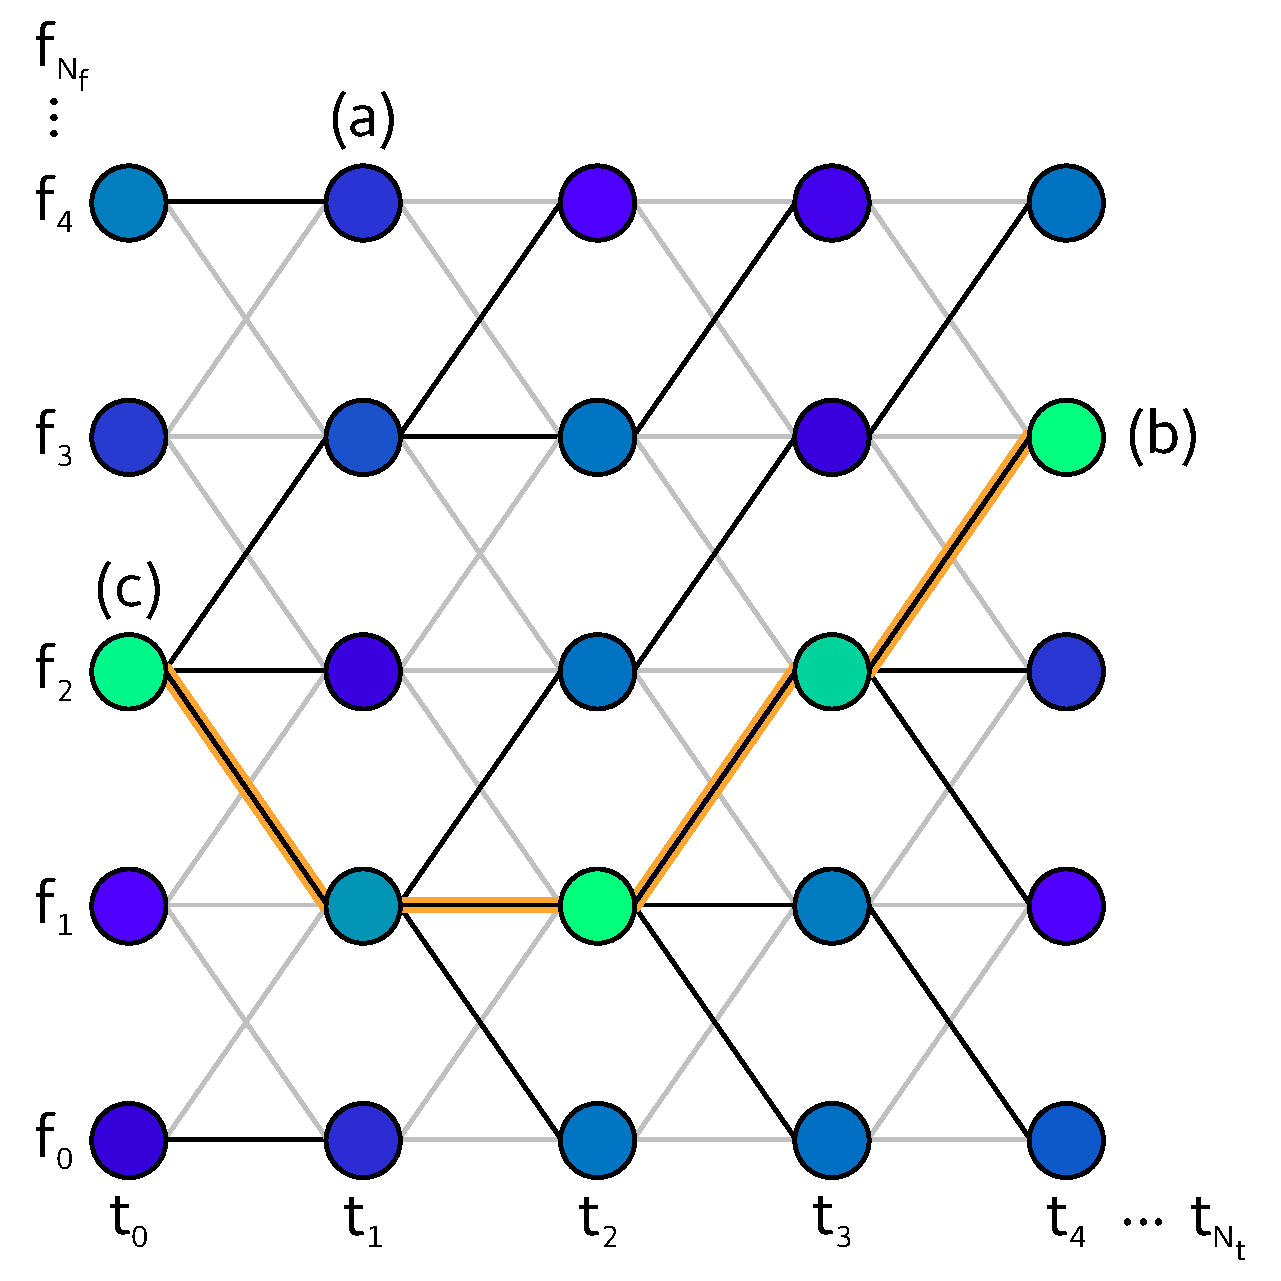
\includegraphics[width=0.49\textwidth]{figures/viterbiDiagramBlue.pdf}
\caption{\label{fig:viterbi}
Schematic diagram of the Viterbi algorithm. 
The circles represent elements in a time-frequency grid, labeled $t_0$ to $t_{N_t}$ (left to right) in time and $f_0$ to $f_{N_f}$ (bottom to top) in frequency. 
The color of each circle represents the likelihood of a signal being present in each time-frequency element.
The dark blue to light green gradient corresponds to low to high likelihood values in arbitrary units for this schematic. 
The objective is to find the most probable path of a signal through the grid from left to right.
All possible paths are shown by the lines. 
The black lines show the best path to each circle and the gray lines show rejected paths. 
Some routes through the grid result in dead-ends with respect to optimally reaching the other side, such as the path ending at $t_1$ marked (a).
At $t=t_{N_t}$ the algorithm chooses the terminating frequency circle which has the highest value given by Eqn.~\ref{eqn:pathprobability}, marked (b). 
The Viterbi path is the path leading to this circle, highlighted in orange from (b) to the start at (c). 
%A schematic diagram of the Viterbi algorithm. 
%Each circle represents an element in the time-frequency grid starting from the instant $t_0$ on the left and ending at $t_{N_t}$ on the right. 
%Vertically, the grid starts from frequency $f_0$ at the bottom and ending at $f_{N_f}$ at the top. 
%The color of each circle indicates the likelihood that a signal is present in the box (the detection statistic), where a lighter color corresponds to a higher likelihood. 
%At each time step, the paths can move up one $f$ bin, move down one $f$ bin, or stay at the same $f$ bin (shown by lines connecting the circles in the diagram). 
%Each circle has three paths leading to it, indicated by the lines. 
%The best path to each circle at each $t_i$ is highlighted in black. 
%Some routes through the grid are found to be dead ends, with respect to optimally reaching the other side, such as the path ending at $t_1$ marked (a). 
%At $t=t_{N_t}$ the algorithm chooses the terminating frequency circle which has the highest value given by Eqn.~\ref{eqn:recursiveViterbi}, marked (b). 
%The Viterbi path is the path leading to this circle, highlighted in orange from (b) to the start at (c). 
}
\end{figure}













The timeseries data from the interferometer is first split into segments. 
We then take the discrete Fourier transform of each timeseries segment to form a grid in time and frequency (a spectrogram) with the Fourier amplitude $F(t_i,f_j)$ as the detection statistic (this is the emission matrix).
Assuming Gaussian noise, this detection statistic choice maximizes the likelihood of detecting a sinusoidal signal as described in Appendix~\ref{app:sinusoid_likelihood}.
The detection statistic is normalized for convenience by dividing each value by the maximum Fourier amplitude in the grid (such that $\max_{i,j} F(t_i,f_j) = 1$).



%The Viterbi algorithm is then applied to the spectrogram data. 
We use the schematic in Fig.~\ref{fig:viterbi} to aid our explanation of the method throughout this section. 
It represents a spectrogram with $N_t$ time bins and $N_f$ frequency bins.
The circles represent the elements of the time and frequency grid, which are labelled as  
$t_i$ and $f_j$ respectively, where $i=0,1,2,...N_t$ and $j=0,1,2,...,N_f$. 
The color of the circles represents the detection statistic $F(t_i,f_j)$ at each grid point where dark blue corresponds to lower values and light green to higher values. 


%The spectrogram schematic, as shown in Fig.~\ref{fig:viterbi}, has $N_t$ time and $N_f$ frequency bins. 
%We label the elements of the time and frequency  grid as $t_i$ and $f_j$ respectively, where $i=0,1,2,...N_t$ and $j=0,1,2,...,N_f$. 
%The normalized Fourier amplitude $F(t_i,f_j)$ is the detection statistic. 


The objective is to find the most likely path through the grid given the observed data and any probabilistic constraints on how the frequency of the signal can wander from $t_i$ to $t_{i+1}$. 
The transition probability matrix, $A(f_k,f_m)$, describes the probability of system transitioning from state $f_k$ at $t_i$ to a state $f_{m}$ at $t_{i+1}$. 
Here, we allow the frequency of the signal to either (a) stay in the same bin, (b) move up by a single frequency bin, or (c) move down by a single frequency bin at each transition A. 
We assign these three transitions equal probability, i.e.\ $A(f_k,f_m)=1/3$ for $k=m+1,m,m-1$ and $A(f_k,f_m)=0$ otherwise.
All possible transitions are shown as lines in Fig.~\ref{fig:viterbi}.
The different colorings of the lines are explained below. 



The signal is equally likely to start in any frequency bin (i.e. the prior is flat). 
We define the probability of the system having frequency $f_j$ at the initial time $t_0$ to be equal to the (normalized) detection statistic at that state (i.e.\  ${\rm Pr}[f(t_0) = f_j] = F[t_0,f_j]$).
A specific path (which may not be optimal) is written as $f(t_0), f(t_1),..., f(t_n)$. 
The probability of a specific path given the data is 
\begin{eqnarray}
{\rm Pr}[ f(t_0), f(t_1),... && f(t_n) | {\rm data}] = \nonumber\\
          && F[t_n,f(t_n)] A[f(t_n),f(t_n-1)] \nonumber \\
          && \times... A[f(t_1),f(t_0)] F[t_0,f(t_0)] \,,
\label{eqn:pathprobability}
\end{eqnarray}
The path $f^\ast(t_0),...,f^\ast(t_n)$ that maximises $Pr[ f(t_0), f(t_1),... f(t_n) | data]$ is the optimal path terminating in the frequency bin $f^\ast(t_n)$. 
We note that there is no marginalization used in this method; the left-hand-side and right-hand-side of Eqn.~\ref{eqn:pathprobability} are both evaluated for a specific path and then we maximize over all such paths to find the optimal Viterbi path. 
%The probability of the system having frequency $f_j$ at any later time $t_{i+1}$ is then defined recursively by
%\begin{eqnarray}
%{\rm Pr}[f(t_{i+1})=f_j] =~& F[t_{i+1},f(t_{i+1})] \nonumber \\
%                     &\times A[f(t_{i+1}),f(t_i)]  \nonumber \\
%                     &\times {\rm Pr}[f(t_i)].
%\label{eqn:recursiveViterbi}
%\end{eqnarray}
%for any path through the grid. 
%The sequence $f(t_0),f(t_1),\dots,f(t_{N_t})$ that maximizes ${\rm Pr}[f(t_{N_t}) = f_j]$ is the optimal Viterbi path terminating in the frequency bin $f_j$. 
%We can then maximize the latter quantity over $0 \leq j \leq N_f$ to find the optimal Viterbi path overall, i.e. terminating in any frequency bin. 


The Viterbi algorithm provides a computationally efficient method for finding the optimal path. 
At every $t_i$ all but $N_f$ possible paths are eliminated (see also Ref.~\cite{ScoX1ViterbiO1:2017}). 
Here we describe the algorithm in pseudocode while referring to the schematic in Fig.~\ref{fig:viterbi}.%, where the circles indicate the elements in the spectrogram with the lighter colors corresponding to a higher likelihood. 
The implementation used in this work is available online (see Appendix~\ref{app:code}).
\begin{enumerate}
\item Starting at time $t_1$, each $f_j$ state can originate from three prior states at time $t_0$ (except for the edge cases $f_0$ and $f_{N_f}$ which only have two). 
The paths between these states are indicated by the lines in Fig.~\ref{fig:viterbi}. 
At each $f_j$ state, we select the path with the highest $A[f(t_0),f(t_1)] {\rm Pr}[f(t_0)]$ value as the most probable path. 
These choices are highlighted using the black lines in Fig.~\ref{fig:viterbi} while the gray lines show the rejected paths. 
For example, the most probable connection to the element labeled (a) is the one directly behind it (i.e., $f_4$). 
Therefore, this path is selected as the best path from $t_0$ to $t_1$ for $f_4$.
To allow backtracking at the end, the index of the most probable connection to a node along with the value of the best path to that node is stored, for each node.

\item Moving to time $t_2$, again, we select the path which maximizes the recursive quantity in Eqn.~\ref{eqn:pathprobability} for each $f_j$. 
These paths are again shown by the solid black lines between the nodes at $t_1$ and $t_2$ in Fig.~\ref{fig:viterbi}.
Rejected paths are again shown by gray lines. 

\item Step 2 is repeated until the end of the grid ($t=t_{N_t}$) is reached with only the best paths being stored at each iteration. 

\item We have now found the most probable path to each $f_j$ at $t=t_{N_t}$ and its probability (Eqn.~\ref{eqn:pathprobability}). 
We select the terminating frequency bin $f(t_{N_t})$ with the highest probability labeled as (b) in Fig.~\ref{fig:viterbi}.

\item The final step is to find the Viterbi path (the overall best path that terminates in the frequency bin with the highest probability in step 4). 
The Viterbi path is found by backtracking along the stored best connections at each $t_i$ (see also Appendix~\ref{app:viterbi}). 
In Fig.~\ref{fig:viterbi}, it is the path ending at (b) that started at (c) highlighted in orange.
%\item The Viterbi path (the overall best path) is then found by backtracking along the stored best connections at each $t_i$ (see also Appendix~\ref{app:viterbi}). In Fig.~\ref{fig:viterbi}, we see that the path ending at (b) started at (c) and is highlighted in orange.
\end{enumerate}

In continuous wave searches, the signal amplitude is expected to be small in comparison to the noise and its frequency could be changing unpredictably over time.
A Fourier transform of the entire dataset splits the signal power between multiple frequency bins and could result in the signal being undetectable under the noise (see Fig.~\ref{fig:viterbi_comparison_webcam_spectrum}). 
The Viterbi algorithm's strength lies in its ability to track such signals through the data.
In the following section, we present the results of using the Viterbi algorithm with the table-top interferometer data. 
% - just simiplifed this discussion a little and added a reference to the CW searches
%The key to the Viterbi algorithm is that we can use the signal's correlation in time to improve the signal-to-noise ratio of the frequency of the wandering signal at a particular time. Since the noise is assumed to not be correlated in time, if the detection statistic at a given frequency is high at a particular time and at neighboring frequencies at neighboring times then the likelihood that the given frequency at that particular time is from the wandering signal increases. By iterating this process through the grid for a suitable choice of the window of neighboring frequencies and times, the Viterbi algorithm is well-suited to finding wandering signals.



% The Viterbi algorithm is an example of a dynamical programming algorithm, where a computation can be broken down into a series of sub-computations.
% The Viterbi path for a time series sequences spanning $t_0$ to $t_{N_t}$ contains the Viterbi path for sub-sequences of that time series. 
% The algorithm is computationally efficient, at every time step all but $N_f$ possible paths are eliminated (see also Ref.~\cite{ScoX1ViterbiO1:2017}).





\subsection{Wandering frequency signal results}
\label{sec:wanderingResults}

\begin{figure*}
	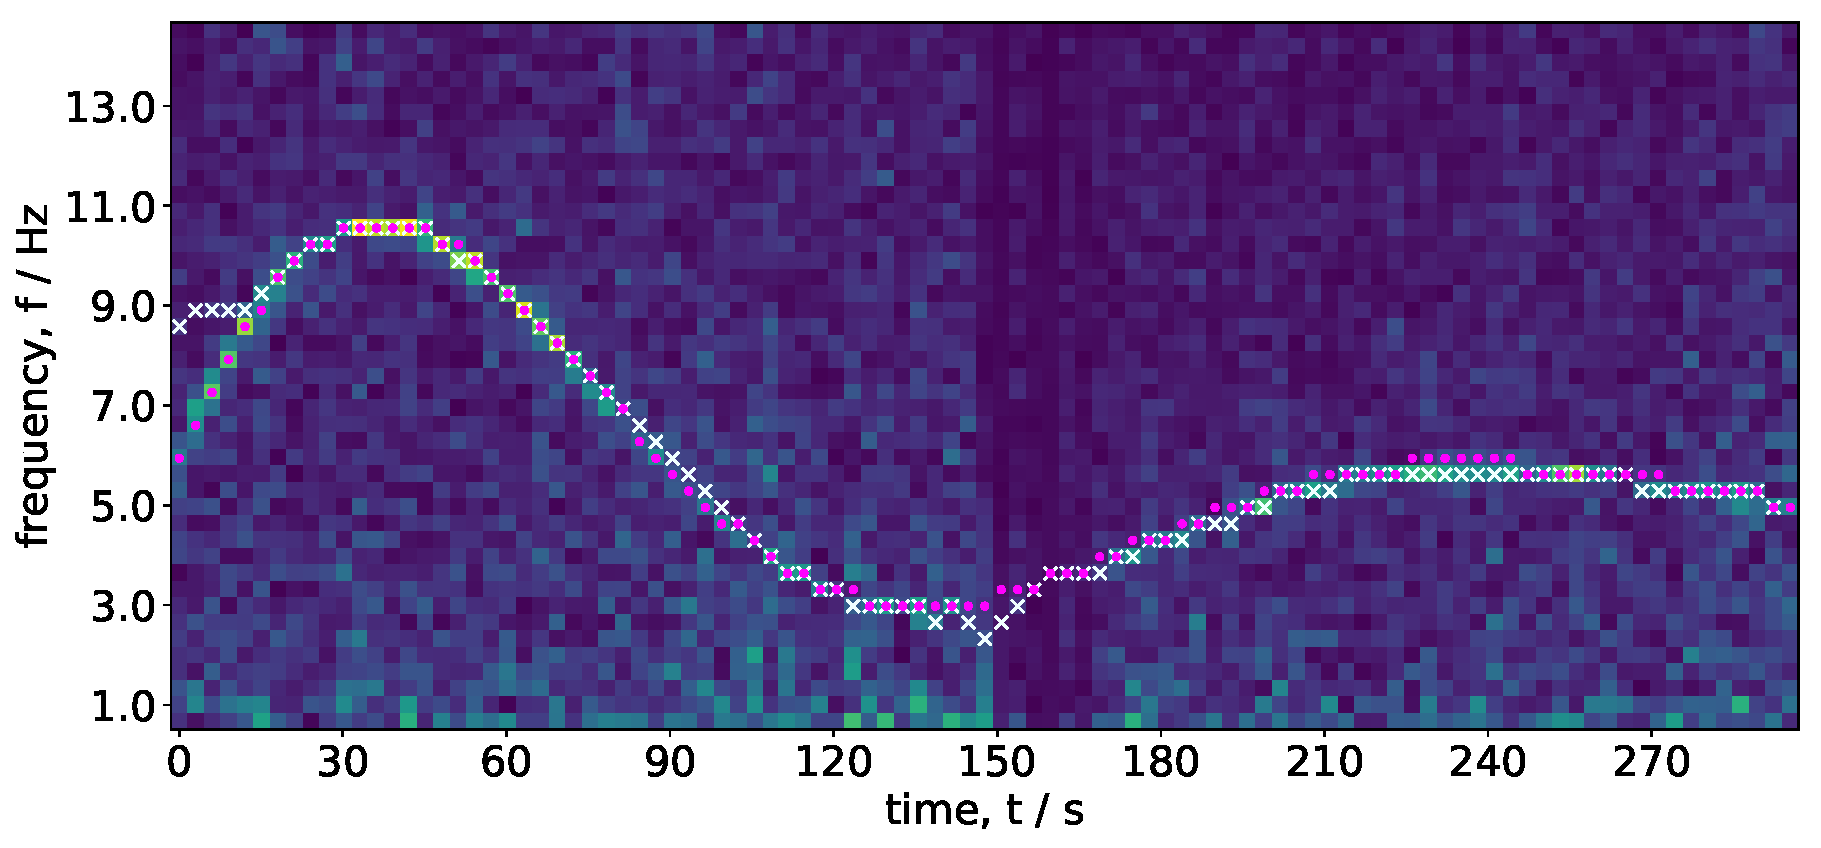
\includegraphics[width=\textwidth]{figures/expt_overlay_2_viterbi_test_webcam.pdf}
	\caption{\label{fig:viterbi_overlay}
Recovery of a wandering tone using the Viterbi algorithm.
The spectrogram (heat-map) coloring indicates the value of the detection statistic (here, the logarithm of the absolute value of the discrete Fourier transform) in each time-frequency bin -- with brighter colors indicating higher values. 
The overlaid pink-dot and white-cross markers show the injected signal and recovered Viterbi path, respectively. 
On the left, before $\sim 15\,{\rm s}$, the signal changes frequency too quickly for the Viterbi algorithm to recover, given a parameter for the rate of change of one frequency bin per time bin. 
At $150\,{\rm s}$ the data appears anomalous, which may be due to some transient background noise. }
\end{figure*}
 

We simulate a slowly wandering signal by modulating the frequency sinusoidally with a modulation amplitude that decays with time. 
We use the same set-up as shown in Fig.~\ref{fig:ifo_schematic_webcam} and the output interference pattern is recorded via webcam as in Section~\ref{sec:single_tone}. 
In this section, we test the Viterbi algorithm’s ability to recover the wandering signal. 
Note that we implicitly approximate the noise at the webcam as white (uniform in frequency) in this implementation of the Viterbi algorithm. 
This approximation ignores the increase in noise at low frequencies (below 1~Hz) shown in Fig.~\ref{fig:webcam_spectrum} but is a reasonable approximation for the higher-frequency (around 5~Hz) wandering frequency signals that we use.



The results are shown in Fig.~\ref{fig:viterbi_overlay}, where the heat-map shows the spectrogram of the observed signal (similar to that represented by the schematic in Fig.~\ref{fig:viterbi}). 
In this demonstration we use a signal that can easily be identified in the spectrogram, however, we expect real continuous-wave signals to have far lower signal-to-noise ratios. 
The overlaid pink dots in Fig.~\ref{fig:viterbi_overlay} show the injected signal and the white crosses show the recovered Viterbi path.
The recovered Viterbi path is within one frequency bin ($\approx 0.3\,{\rm Hz}$) of the injected signal for $94\%$ of the time. We also compute the root-mean-square (RMS) fractional error $E_{\rm rms}$ along the path, which is defined as 
\begin{equation}
E_{\rm rms} = \left[ \frac{1}{N_t+1} \sum_{i=0}^{N_t} \frac{(I_i - R_i)^2}{{I_i}^2} \right] ^{1/2}\,,
\end{equation}
where $I_i$ and $R_i$ are the injected and recovered (Viterbi) frequency paths, respectively. 
For the result shown in Fig.~\ref{fig:viterbi_overlay}, we find that $E_{\rm rms} = 0.082$, which indicates fair but not total recovery of the injected signal.


This may be explained by two anomalies in the recovered path. Initially, the injected signal wanders by more than one frequency bin per time bin (i.e.\ faster than the algorithm is allowed to), thus leading to a discrepancy between the injected and recovered paths for $t\lesssim 10\,{\rm s}$. One may be tempted to increase the allowed frequency wander in the algorithm, however, this leads to an overall decrease in the above statistics, as the algorithm is prone to jump briefly to nearby spots of noise. There is also an anomaly at $150\,{\rm s}$, which is likely due to a local disturbance, e.g. someone walking past the interferometer. 
As shown in Fig.~\ref{fig:viterbi_overlay}, the Viterbi algorithm can recover and continues to track the signal after the disturbance. 
%The Viterbi algorithm is somewhat robust against such disturbances, qualitatively recovering the injected path on the other side, as shown in Fig.~\ref{fig:viterbi_overlay}. 



\end{document}
